\chapter{\sc Tools for surface Science}
\label{ch:Tools for surface Science}
%\graphicspath{{/Users/LionsTiger/Dropbox/research/thesis/UNH_eThesis_Template/figs/}}


% --- Insert Text --- %
\section{Low Energy Electrons - Ideal Surface Science Probes}
Many different tools exist for probing and characterizing the structure crystalline materials. Photons, electrons, ions, and atoms can all be used for different purposes when analyzing various properties of a material. Of these probes, low energy electrons are uniquely equipped for the analysis of precise atomic locations within the surface region of a material. This fact is attributed to their very short mean free path. The mean free path of an electron in a material depends on the energy of the incident electron. The dependence of electron mean free path on the electron kinetic energy is shown in Figure \ref{fig:univ-curve}, which is known as the universal curve for electron mean free path in solid materials. From this figure it can be seen that low energy electrons provide an ideal probe of material properties at the surface due to the fact that the mean free path covers at most only a few atomic layers, thus low energy electrons are highly surface sensitive. This extreme surface sensitivity is what allows Auger Electron Spectroscopy, AES, to provide precise chemical analysis of a crystal surface region. This tool is primarily used for measuring the relative level of surface contamination when preparing surface for experimental analysis.

\begin{figure}
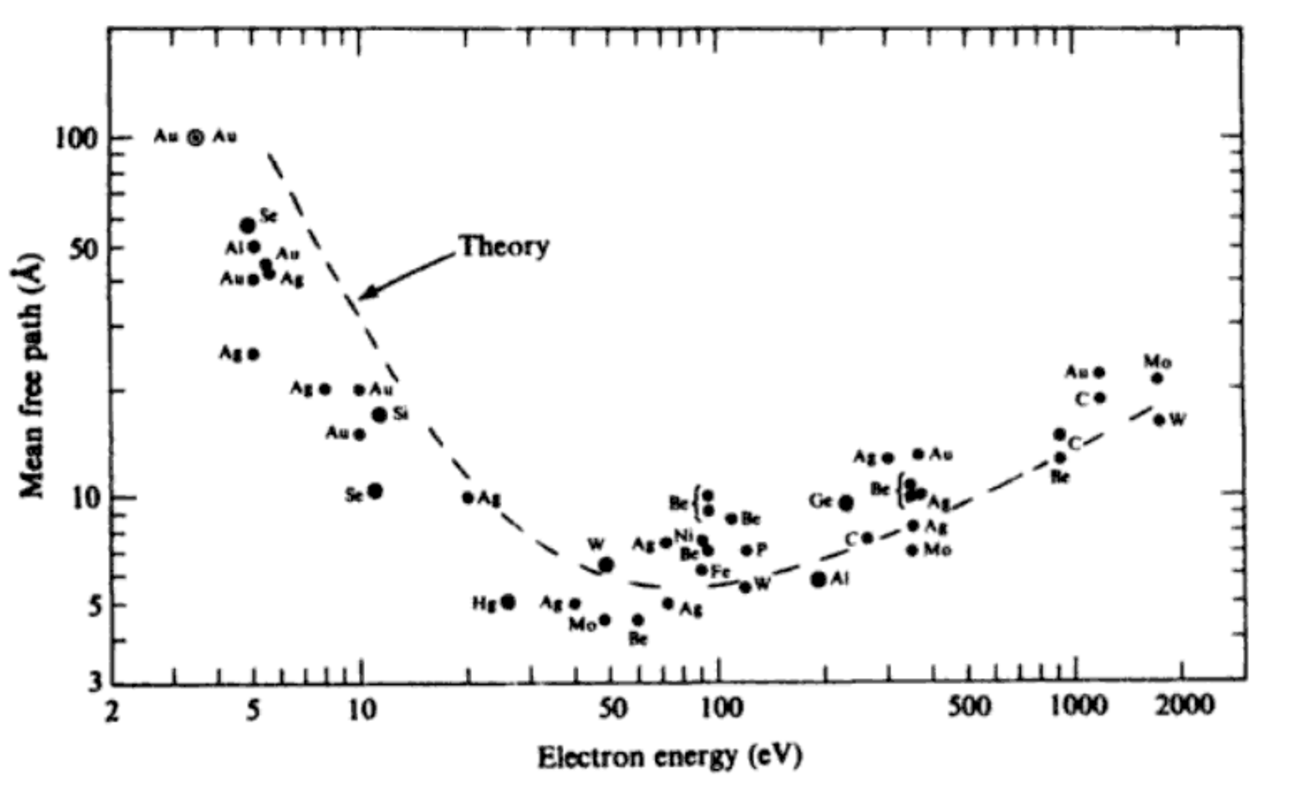
\includegraphics[scale=0.35]{figs/universalcurve.png}
\caption{Universal curve of electron mean free path in solids \cite{Zangwill}}	
\label{fig:univ-curve}
\end{figure}

\section{Low Energy Electron Diffraction}
When investigating the structure of bulk solids, diffraction is generally the most important tool; both photons and electrons are readily used as diffraction based probes of atomic structure. Analysis of diffraction through solid materials provides direct information about any translational or rotational symmetry present in the target material and thus can be easily used to characterize the structure of periodic crystalline materials. The study of crystallographic structure of materials dates back to the work of L. Bragg in 1913, who founded the field of X-ray crystallography \cite{Ashcroft}.

Crystalline solid materials exhibit high degrees of atomic ordering in three-dimensions with a specific periodicity in one or more directions. The surface of the solid represents a deviation from perfect infinite periodicity. Ideally the surface retains the same periodicity of the bulk solid structure, however, more often than not, the surface structure of a material contains significant deviations from the bulk structure. These geometric changes in atomic structure may result in interesting physiochemical changes in the material and thus are of particular interest for study.

\begin{equation}
\label{eq:lat}
\mathbf{R} = n_1 \mathbf{a_1} + n_2 \mathbf{a_2} + n_3 \mathbf{a_3}
\end{equation}


Solid materials can be described by the symmetry of their atomic structure. The Bravais lattice defines a purely geometric periodic array of lattice sites that house the repeated structure of the solid be that a single atom, group of atoms, or molecules. Equation \ref{eq:lat} defines the bravais lattice as all points with position vector, $\mathbf{R}$, with $\mathbf{a_n}$ representing basis vectors and  $n_n$ taking integer values \cite{Ashcroft}.

\begin{equation}
\label{eq:rlat1}
\mathbf{ b_i \cdot a_j} = 2\pi \delta_{ij}
\end{equation}

\begin{equation}
\label{eq:rlat2}
\mathbf{b_i} = 2\pi \frac{\mathbf{a_j \times a_k}}{\mathbf{a_i \cdot (a_j \times a_k)}} \text{  }\forall \text{ cyclic permutations of ijk}
\end{equation}

For every lattice defined by the set of primitive basis vectors, ${\mathbf{a_n}}$, there is a corresponding set of reciprocal lattice vectors, ${\mathbf{b_n}}$,  that generate the reciprocal lattice of the real space lattice.  These vectors have units of inverse length and thus can be considered to be the momentum space representation of the real space lattice. The reciprocal lattice plays a role in governing crystalline diffraction and a generalization of the law of conservation of momentum to discrete periodic lattices \cite{Ashcroft}. The reciprocal lattice basis vectors, ${\mathbf{b_n}}$, must satisfy the relations shown in Equations \ref{eq:rlat1} and \ref{eq:rlat2}. That the reciprocal lattice contains the same symmetry as the original real space lattice makes diffraction techniques, which are sensitive to the reciprocal lattice, able to provide real space information about precise atomic positions in the crystal.

Low energy electrons are distinctly qualified to probe the surface structure in solids for two primary reasons. First, as shown in Figure \ref{fig:univ-curve}, low energy electrons have minimal mean free path and thus will interact only with the first 3-5 atomic layers in a material. Finally the deBroglie wavelength of the electron is comparable to the interatomic distance in most solids, which allows for diffraction.

Electron diffraction is analogous to the theory of X-ray diffraction first described by L. Bragg, and is governed by the Laue equation, shown in Equation \ref{eq:laue}, describing the total change in wave vector of an electron after scattering. Here $\mathbf{K_{i}^{||}}$ and $\mathbf{K_{s}^{||}}$ represent the components of the wave vectors of the incident and scattered electrons parallel to the crystal surface and $\mathbf{g_{hk}}$ represent a reciprocal lattice vector of the crystal at the reciprocal lattice point denoted by (hk). The Laue condition then demands that in an electron scattering event, the total parallel component momentum transferred must be equal to a reciprocal lattice vector of the crystal. Using the Planck-Einstein relation for energy, the condition for elastic scattering, $E_i = E_s$, reduces to $|K_i| = |K_s|$. Here its worth nothing that the conservation of momentum, as implied by the Laue condition, $K_s^{||} = K_i^{||} - g_{hk}$ applies to electrons of any source, thus this condition describes the kinematics for low energy electron diffraction, Auger electron spectroscopy, as well as photoemission spectroscopy \cite{ SurfSciTechniques}. 

\begin{equation}
\label{eq:laue}
\Delta \mathbf{K^{||}} = \mathbf{K_{s}^{||} - K_{i}^{||}} = \mathbf{g_{hk}}
\end{equation}

The patterns formed by electron diffraction represent a scaled version of the reciprocal space lattice of the target crystal and thus contain information about translational and rotational symmetry in the real space system by the inverse transformation correlated with Equations \ref{eq:rlat1} and \ref{eq:rlat2}. While it is relatively straightforward to use LEED to derive the symmetry of the target crystal surface structure, it becomes more difficult to extract information regarding precise atomic positions relative to those predicted for the bulk structure. For this a more complex method of diffraction data analysis is employed, known as dynamical LEED intensity-voltage analysis, LEED-I(V).

In LEED-I(V), the energy of the incident electron beam is varied in discrete steps and the intensity, I, of various diffracted beams is analyzed as a function of the incident energy, V. This process requires additional hardware to capture images of the diffraction pattern for each step in energy of the incident electron beam, but the data extraction is relatively straightforward. For each energy step, an image of the diffracted beams is captured and saved digitally. One or more diffracted electron beams are selected in the images with an adjustable sized rectangular integration window. The total intensity of the beams in the window is summed and recorded. Finally this intensity is plotted as a function of the energy range of the experiment; optionally a local background can be subtracted from each data point for more accurate data. These intensity-energy curves contain information about the three dimensional structure of the diffracting material \cite{Hannon-LEEM-Book, vanHove-LEED, pendry-LEED}. 

In order to derive the atomic structure of the target material, a three -dimensional trial structure is provided to software packages that calculate the dynamic multiple scattering of incident electrons and predict the diffracted intensity as a function of incident energy. This computationally generated I(V) curve is then compared to the experimentally gathered I(V) curve. Then the trial structure is adjusted slightly and the process continues to iterate until reasonable agreement is found between the experimental data and computationally generated data. The last structure input to the process then contains the most accurate information about three-dimensional atomic positions in the target crystal. This structure can be compared to that of the known bulk crystal structure to analyze the presence of surface reconstructions and relaxations.


\section{Low Energy Electron Microscopy}
Low energy electron microscopy is a novel technique for rapid and robust surface science analysis. Electron microscopy dates back to the early 1930s and has evolved into a wide variety of analytic techniques. LEEM is a subset of cathode lens electron microscopy developed in principle in the 1960s while not fully realized until the 1980s after technological advances in vacuum technology and electromagnetic lens systems for electron optics. There are two primary features of LEEM that distinguish it from other forms of cathode lens microscopes, namely the energy regime of the incident beam and usage of the sample specimen as part of the lens system itself \cite{Hannon-LEEM-Book}.

LEEM can generally operate in two distinct modes by varying the probing source. In photoemission electron microscopy, (PEEM), a collimated beam of monochromatic photons is used to probe the sample surface and images of the surface are generated from photo-excited electrons. In LEEM mode, a collimated beam of low energy electrons in the range 0 to 100 eV is used to probe the surface region of the sample specimen. Analogous to LEED, low energy electrons are chosen specifically due to their high surface sensitivity as a direct result of their low mean free path. However, using low energy electrons as the primary beam poses many technological challenges. 
Lower energy electron beams are more susceptible to influence by external stray electromagnetic fields, which makes the electron beam difficult to control over large distances. To get around this challenge LEEM uses a high-energy electron beam in the range of 15 to 20 keV as the primary beam. The high-energy beam can be easily focused and manipulated using electromagnetic lenses.  The incident electron beam is only decelerated to very low energies just prior to interaction with the sample. This is accomplished by integrating the sample with the cathode lens. After passing through the objective lens, the high-energy electron beam experiences an approximately uniform retarding electric field from the cathode, which lowers the beam energy to the 0 to 100 eV range. The sample must be held at a high negative bias potential while simultaneously the space between the sample and objective lens must be very small in order to generate a strong electric field on the order of $10^6$ volts per cm \cite{Hannon-LEEM-Book}.

Using the sample as part of the cathode lens primarily restricts the types of samples available for study to non-insulating samples that are approximately flat. A sample that is overly rough or warped will cause the retarding field to be non-uniform thus reducing the overall resolution in the system as well as providing potential for sparks in the optics system between sample and objective lens. The high field requirements, sample conductivity, and macroscopic flatness prove to be minimal restrictions considering the advantages offered by LEEM analysis.

One of the most robust aspects of LEEM analysis is the ability to provide one tool that can image the sample in both real space and reciprocal space with high resolution. The objective lens of the LEEM system provides two focal planes that can be projected into the imaging column of the detection system. While operating in standard LEEM mode, the Gaussian plane of the objective lens provides a real space image of the sample surface with resolution better than 10nm parallel to the surface plane \cite{Hannon-LEEM-Book}. The back-focal plane of the objective lens can also be projected to the imaging column. This provides a direct image of the diffraction pattern or, said another way, records the angular distribution of the diffracted electron beams \cite{Hannon-LEEM-Book}.  Similarly in PEEM mode the Gaussian plane again provides a real space image generated by photo-emitted electrons, whereas the back-focal plane provides an image of the angular distribution of the photoemission process.

Reciprocal space images collected with a LEEM system are useful and distinct from conventional LEED imaging as a result of being able to drastically restrict the size of the incident electron beam. By introducing a limiting aperture into the illumination column, the spot size of the imaging beam can be restricted to sub-micron levels. To contrast this with conventional LEED, generally the illuminated area of the sample in conventional LEED spans multiple square millimeters \cite{Hannon-LEEM-Book}.
	
A second unique design in LEEM systems is the use of magnetic prisms to separate the incident and reflected electron beams by angular deflections. This allows the sample to be removed from the electron beam directly emitted from the electron source. In other words the sample is not required to be collinear with the electron source. This gives rise to a number of possible beam line geometries. An example of a standard LEEM beam line geometry is shown in Figure \ref{fig:LEEM-Geometry}. Having the sample removed from the direct line of sight of the electron source while also separating the incident and outgoing beams allows imaging of all reflected beams. 

In conventional LEED, the (0,0) spectrally reflected beam is not visible on the luminescent screen due to being blocked from view by the electron source. LEEM allows the spectral beam to be imaged directly along with emitted beams of higher angular order, however, in real space imaging, the surface image can only be formed by one  reflected beam at a time. Having the sample separated from direct line of sight with clever beam-line geometries allows LEEM to be implemented alongside other incident beams such as a molecular flux from a molecular beam epitaxy system (MBE). Thus LEEM can be used to image the real-time growth of thin films of a wide variety of materials atop a wide variety of substrates. This fact alone makes LEEM incredibly powerful and useful in the field of surface science. 
\begin{figure}
\centering
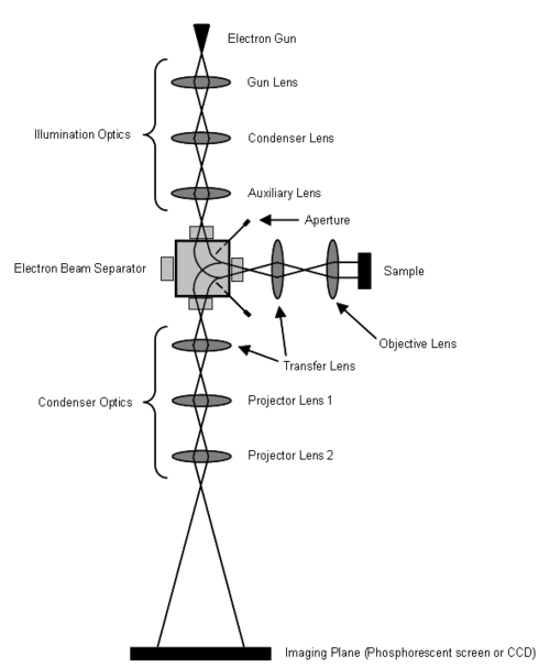
\includegraphics[scale=1.1]{figs/LEEMGeo-150.png}
\caption{Diagram of basic LEEM geometry. The sample is oriented at $\pm$90$^{\circ}$ with respect to the beam emitted from the electron source. Source from Brandon Howe: \protect\url{https://en.wikipedia.org/wiki/Low-energy_electron_microscopy}}
\label{fig:LEEM-Geometry}
\end{figure}
	
	The primary limits on the resolution in LEEM imaging come from aberration in the electron optics. The objective lens must have a small uniform aperture cut into its center in order to allow the incident and reflected beams to pass through it. This hole causes the field generated by the cathode to deviate from a ideal uniform field. Fringe effects from the aperture cause a divergence of the reflected beam after passing through the objective aperture. These aberrations are well understood and can be partially corrected through the use of an extra aberration correction that involves the installation of a second magnetic beam separator. This adds a significant cost to the device, yet also allows for an ultimate in-plane spatial resolution as low as 2 nm \cite{Hannon-LEEM-Book, Figuera-LEEM}. 

As LEEM continues to evolve as a powerful surface science tool, novel experimental techniques push the boundaries of LEEM's ultimate resolution while also granting access to new types of samples for imaging. By altering the electron source to provide polarized electrons, which have a fixed spin orientation, the magnetic domains in the sample surface can be probed with very high spatial resolution. This technique is known as Spin Polarized LEEM, SPLEEM. LEEM, along with many other electron microscopy methods, has a long history in the study of biological specimens \cite{Bauer-LEEM}. As biologic sciences advance, the need for rapid characterization techniques grows. One of the fundamental problems in modern biological science is characterization and sequencing of DNA samples in a rapid manner. This technique requires the ability to distinguish between different base pairs existing in individual DNA strands and is currently a cost-prohibitive technique \cite{MADLEEM}. A novel LEEM technique using a monochromatic aberration-corrected dual-beam LEEM system, (MADLEEM), seeks to utilize the high spatial resolution of LEEM to rapidly sequence DNA samples \cite{MADLEEM}.

LEEM's high spatial resolution within the plane of the sample surface can be extended to provide three dimensional mapping of atomic positions in the surface region through use of LEEM-I(V). LEEM-I(V), analogous to LEED-I(V), combines experimental data with computational modeling of dynamic electron scattering to generate a model of the atomic surface structure with very high resolution. Real space LEEM images represent maps of the local electron reflectivity in the surface. As the incident electron energy is changed, the local electron reflectivity also changes in ways uniquely linked to the physical and chemical properties of the local surface region.

LEEM-I(V) requires computational modeling to discern accurate information about the surface structure. A complicating factor for computational modeling of very low energy electron interactions is the treatment of the electron inner potential. For higher energy than LEEM operates at, the potential can be assumed constant. For very low energies, however, there is a complex energy dependence. Dynamical modeling of low energy electrons is an active area of current research. 

LEEM-I(V)  techniques are currently under study as a method for discerning the number of atomic layers in a sample with a high degree of spatial accuracy. This is useful for the study of novel layered materials such as graphene and other two-dimensional materials. As a result of thin film interference and/or quantum well resonance, the I(V) curves for layered materials show oscillations in the reflected intensity. These oscillations are inherently linked to the thickness of the material and thus to the number of layers \cite{Hibino}. Thus careful analysis of LEEM-I(V) data can elucidate the sample thickness for layered materials. This form of analysis, alongside software written to aid in data visualization and I(V)  data extraction, will be shown later as applied to a novel graphene system under study at UNH.
	
	
\section{Scanning Tunneling Microscopy: Ultra High Resolution Surface Microscopy}

STM is a form of non-optical scanning probe microscopy, which provides detailed mapping of the topography of a surface with atomic resolution. The mechanism of action, while relatively simple, relies on a purely quantum phenomenon called quantum tunneling, and thus STM has no classical analog. 

STM generates images by moving a finely pointed metal electrode across a sample while keeping the electrode-sample distance very small, on the order of a few Angstr\"oms. When a small bias voltage is applied between the STM tip and the sample, then electrons flow from tip to sample or sample to tip through the classically forbidden vacuum region. Classically, if the sample and tip are not touching then there is no flow of electrons due to not having a closed circuit. However, when the separation between tip and sample becomes so small that quantum physics begins to play a role, a current can flow whereby electrons tunnel through the vacuum region.

The amount of current crossing the classically forbidden region is exponentially dependent on the tip to sample distance. Thus, when the tip is closer to the sample surface more current flows and the opposite is true for larger tip to sample distances. Careful monitoring of the tunnel current coupled with the ability to precisely control the tip to sample distance via piezoelectric motors and a computer controlled feedback loop allows the STM to continuously read out a constant current. As the STM scans across the surface, the tip moves perpendicular to the surface plane so as to keep the tunnel current at a constant value. Thus the tip motion essentially traces out the topography of the sample surface; if the tip to sample distance is collinear with the z direction then the sample surface is in the x-y plane and the STM tip motion as a function of the position is a three-dimensional map of the surface structure, $z(x,y)$.

The simplest way to model the operation of an STM considers electrons tunneling through a one-dimensional barrier. The tip and surface can be considered for simplicity as two parallel metallic electrodes. The parameters needed to characterize the tunneling phenomenon in this model are the barrier height, $V_0$, the tip to surface distance, $s$, and the electron energy, $E$. Inside either of the two electrodes, the electron wavefunctions take on the form of traveling waves in the direction perpendicular to the surface plane, $z$, and are proportional to $e^{\pm i z}$. The vacuum region, represented by the one-dimensional potential barrier, is the classically forbidden region. In this region the electron wavefunction must decay, and thus the wavefunction inside the barrier region is represented by $e^{\pm \kappa z}$. Solving the Schr\"odinger equation yields the following relations for $k$ and $\kappa$ \cite{SPM-methods}:
\begin{equation}
k = \frac{[2 m_e (E - V_0)]^{\frac{1}{2}}}{\hbar}
\end{equation}
\begin{equation}
\label{eq:stm}
\kappa = \frac{[2 m_e (V_0 - E)]^{\frac{1}{2}}}{\hbar}
\end{equation}
Continuing the calculation and solving for the probability of an electron tunneling through the barrier yields the following exact solution for the transmission coefficient, $T$,\cite{SPM-methods}:
\begin{equation}
T = [1 + \frac{(k^2 + \kappa^2)}{(4k^2 \kappa^2)} \sinh^2{(\kappa s)}]^{-1}
\end{equation}
Taking the limit that the vacuum region should be strongly attenuating, i.e. $\kappa s >> 1$, the transmission coefficient simplifies to a more understandable term \cite{SPM-methods}:
\begin{equation}
\label{eq:stm2}
T \approx \frac{16k^2\kappa^2}{(k^2 +\kappa^2)^2}e^{-2\kappa s}
\end{equation}
In the approximate form for the transmission coefficient, it can be seen that the probability of an electron tunneling through the barrier depends exponentially on the tip to surface distance, s. Thus an STM can make high resolution maps of the surface by monitoring small changes in the tip to sample distance, which in turn cause large fluctuations in the tunneling current. A change of the tip to sample distance of 1{\AA} can cause a change in the measured tunneling current by roughly an order of magnitude \cite{SPM-methods, BinnigRohrerSTM}.

While the STM data can be considered a topographic map of the surface, the STM actually acts as a probe of the local density of electronic states in the surface. Depending on the direction of the bias voltage applied between the tip and sample, electrons will either tunnel from the sample into the tip or the tip into the sample. In the first scenario, electrons tunnel from the sample to the STM tip; electrons from the highest occupied electronic states in the sample will tunnel into the STM tip filling the lowest unoccupied electronic states. In this case the STM image represented by $z(x,y)$ provides a three-dimensional map of the local density of the highest occupied electronic states in the sample. In the second scenario, electrons from the highest occupied electronic states in the STM tip tunnel into the lowest unoccupied electronic states of the sample. Thus the STM image represented by $z(x,y)$ now provides a three-dimensional map of the density of lowest unoccupied electronic states in the sample surface region. The magnitude of the applied bias voltage affects also affects which electronic states are capable of contributing to the total tunnel current \cite{STM-I}. STM tips are generally chemically etched such that they are as sharp as possible. The tip sharpness and the high sensitivity of tip to sample distance make STM a uniquely local probe. These two characteristics combine to allow the ultra high-resolution surface structure measurements.

The tip to sample distance is an important factor in why STM images provide high spatial resolution. Since the probe of the surface is an electron, one should consider the wavelength of the electron at a typical energy for STM operation to understand limits of resolution. However, since STM operates with tip to sample distances on the order of a few {\AA}ngstr\"oms, this distance is less than that of the electron wavelength. For example using the relation between the de Broglie wavelength in Angstr\"oms and electron energy in electron volts, 
\begin{equation}
\lambda(E_{eV}) = \frac{12.3}{E^\frac{1}{2}} {[\text{\AA}]}
\end{equation} you find for a 1.5eV electron a wavelength of roughly 10 {\AA} \cite{Ashcroft}. This wavelength would in general not allow for resolution of any surface features smaller than the wavelength, such as atomic separation distances, which are on the order of 3{\AA}. STM is not bound by the Fraunhofer diffraction limit of electron wavelength because the tip to sample distance is lower than the electron wavelength \cite{SPM-methods}, and thus the STM operates in the near-field regime.  This makes STM uniquely qualified as a microscopy technique for detailed structural analysis requiring atomic precision.

Besides providing topographic information of the sample surface, STM can collect data in a number of other operational modes. Equations \ref{eq:stm} and \ref{eq:stm2} demonstrate the functional dependence of the tunneling current on the local tunneling barrier $V_0$. The local tunneling barrier is related to the work function of the two electrodes in the tunneling system. Thus STM can be used to investigate changes in work functions of materials at a highly local scale \cite{STM-I}. STM is also frequently operated in one of a number of spectroscopic modes known as scanning tunneling spectroscopy, STS. As mentioned previously, the local tunneling barrier height is related to the tip to sample distance and also the work functions of the two electrodes. By scanning the tip across the sample but at each sampling point also collecting a measurement of current as a function of tip height for varying values of the tip height, then the local tunneling barrier can be extracted from a semilog plot of tunneling current versus tip to surface distance.
\begin{equation}
\label{eq:stm3}
I \propto \int_{0}^{eV} \rho(E) T(E,V) dE
\end{equation}

Many modes of spectroscopic operation for STM have been developed. Generally these modes seek to decouple the geometric and/or topographic information in the STM images from the electronic information. STS allows information about the density of electronic states to be recorded more accurately by recording how the tunnel current changes with bias voltage as a function of bias voltage, $\frac{dI}{dV}(V)$. This quantity is proportional to the density of states in the surface region to first order \cite{SPM-methods}. While many different STS techniques are capable of elucidating the electronic properties of the surface, they come with added drawbacks. STS experiments that map the electronic structure of the sample surface as a function of energy and spatial position require repeated scans of the exact same area of the surface with high precision. This makes thermal fluctuations in the system as well as chemical changes to the scanning probe incredibly important to control \cite{SPM-methods}. Thus extracting spectroscopic data generally requires a low temperature STM, well prepared samples, well prepared tips, and excellent vacuum conditions.


However, if one is only concerned with analysis of the general topographic structure of the sample surface region, then low temperatures are not needed and standard STM images provide the needed information. The work detailed later utilizes room temperature STM to analyze the surface structure of a novel graphene system in comparison to the well-known structure of graphene grown epitaxially on the ruthenium surface.

\section{Further Surface Science Techniques}
Before a sample is ready to study with STM, the surface must be adequately prepared and characterized to ensure that it is free of contamination. One of the major limitations of STM is the lack of distinct chemical sensitivity. While STM images may display surface defects and surface contaminants in the form of adatoms or clusters of atoms, there is no direct signal to specify the type of atom being imaged. Auger Electron Spectroscopy is a surface sensitive technique, which measures the relative elemental composition in the surface region. By illuminating the surface with a collimated beam of electrons, electron emission from the surface can be stimulated as a result of the Auger scattering process. This process can be modeled in three steps. 

The first step is ionization of an atom by the incident electron beam. Here so long as the incident beam has sufficient energy, $E \approx 2keV$, a core level electron in the surface atom will be emitted. Since the first step results in an excited electronic state for the surface atoms, the second step is relaxation. Here a higher shell electron will transition to the core vacancy. The final step is Auger emission. In this step the transition energy of step two is imparted to another non-core electron in the surface atom. If this energy is larger than the electron binding energy, the second electron will be emitted from the atom as a free electron.

The Auger process clearly requires atoms with multiple electrons, thus as a result, Auger Spectroscopy is insensitive to hydrogen and helium. The Auger process can be characterized by the electron level of the core electron and the two levels of the higher shell electrons. The process is denoted using the spectroscopic notation for the energy levels involved, thus for example, a common Auger process involves a core electron from the K energy level and two electrons from the L energy level and is denoted as a KLL transition. The kinetic energy of the emitted electron can be calculated as $E_K - (E_{L1} - E_{L2})$ where $E_K$ is the energy of the core electron, $E_{L1}$ is the energy of the electron that fills the core vacancy, and $E_{L2}$ is the energy of the emitted electron's energy level.

Since the energy of the emitted electron depends on the exact energy levels of the atom it came from, the kinetic energy of the electron contains chemical information. Thus by illuminating a sample with a collimated beam of electrons and carefully measuring the energy of emitted electrons, the elemental composition of the surface can be accurately measured to within a few percent. This is extremely beneficial when preparing a sample for further analysis via LEED and STM. An example of the Auger spectrum recorded from a ruthenium crystal is shown in Figure \ref{fig:auger-ru}.

\begin{figure}
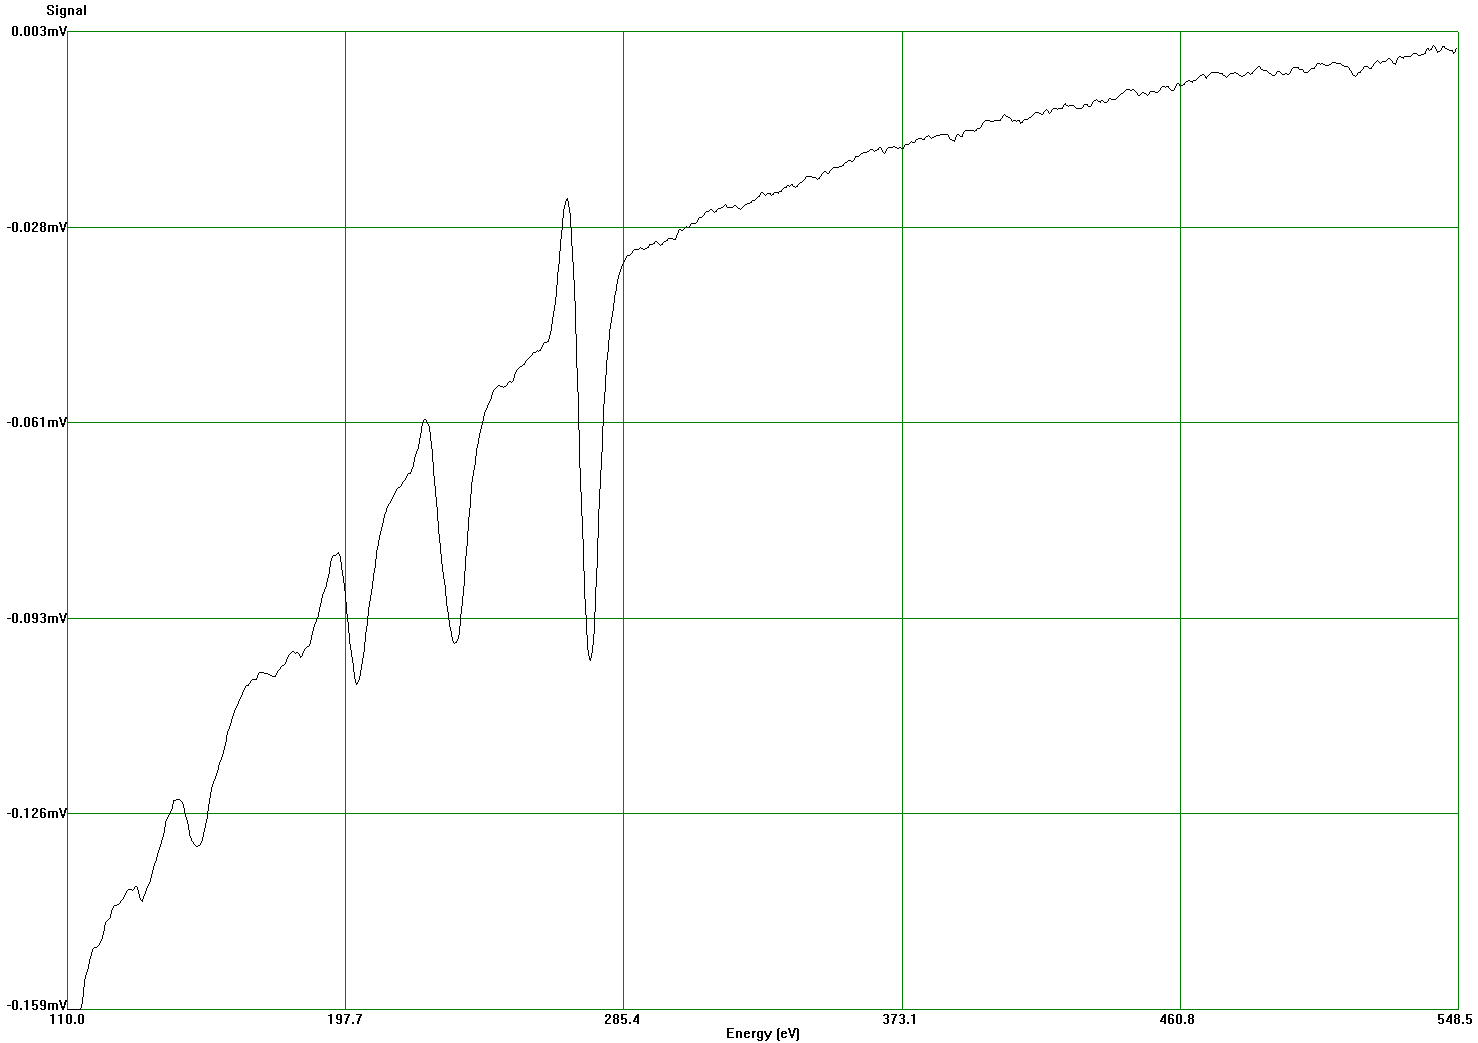
\includegraphics[scale=0.42]{figs/auger-ru.png}
\caption{
An example auger electron spectrum collected from a ruthenium single crystal. The peak at 272 eV is the primary peak for the ruthenium auger spectrum. The primary electron energy is 1.5 keV.
}
\label{fig:auger-ru}
\end{figure}

\section{Summary}
The following surface science studies of a novel graphene system and other layered materials make use of the following tools: AES for characterization of the sample contamination levels, LEED for characterizing the crystalline properties of the sample at the macroscopic scale, STM for analyzing the surface topography at the nanoscale and finally LEEM and micro-LEED to analyze the structure of the surface with high resolution to better understand the atomic structure and layer thickness.

% ------------------- %